
\begin{figure*}[t]

    \begin{subfigure}[t]{0.42\textwidth}
        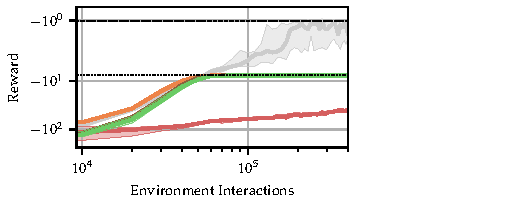
\includegraphics[width=0.95\textwidth]{figures/sec4/cr/lg/sec4_representation_IceLake_True_cr_logs_LavaGap_LavaGapCompiledRun_.pdf}
        \caption{Frozen Lake.}
        \label{supp:fig:grid:a2dplot_2:lg}
    \end{subfigure}%
    %
    \hfill%
    %
    \begin{subfigure}[t]{0.42\textwidth}
        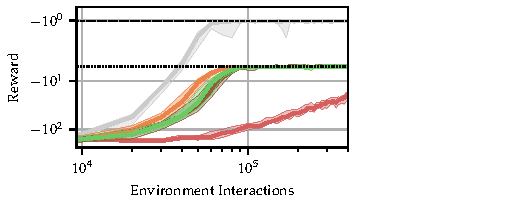
\includegraphics[width=0.95\textwidth]{figures/sec4/cr/td/sec4_representation_TigerDoor_True_cr_logs_TigerDoor_TigerDoorCompiledRun_.pdf}
        \caption{Tiger Door.}
        \label{supp:fig:grid:a2dplot_2:td}
    \end{subfigure}%%
    %
    \hfill%
    %
    \begin{subfigure}[t]{0.15\textwidth}
        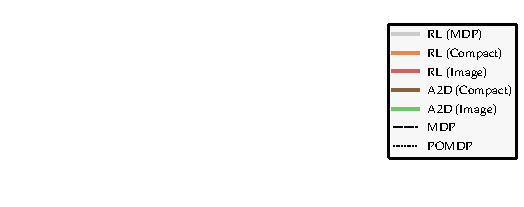
\includegraphics[width=0.95\textwidth]{figures/sec4/legend_representation.pdf}
    \end{subfigure}%

    \caption{Training curves comparing convergence of A2D and vanilla RL on the POMDP for compact (one-hot vector) representations and image-based representations.  We see that RL on the compact partial representation (orange) converges to the optimal POMDP reward (horizontal dotted line, $-9 \times 10^0$ and $-7 \times 10^0$) quickly, and in a sample complexity similar to the best-case convergence of RL in the MDP (gray), which converges to the optimal MDP reward (horizontal dashed line, $- 1 \times 10^0$), when both use hyperparameters comparable to as were used with A2D.  In contrast, RL on the images (red) converges slowly, and does not reach the optimal POMDP reward within the allocated computational budget.  A2D on the other hand converges to the optimal POMDP reward in a sample complexity commensurate with RL operating directly on the compact representation, for \emph{both} image-based and compact representations (brown and green respectively).  This confirms our hypothesis that A2D can reduce the complexity of operating in high-dimensional, partially observed environments to a complexity commensurate with the best-possible convergence rate obtained by performing RL directly on the most efficient encoding or complete state.  { }
    }
    \label{supp:fig:grid:a2dplot_2}
\end{figure*}